\documentclass[10 pt,usenames,dvipsnames, oneside]{article}
\usepackage{../../../modelo-ensino-medio}



\begin{document}

\begin{center}
  \begin{minipage}[l]{3cm}

\includegraphics[width=2cm]{logo}    
\end{minipage}\hfill
\begin{minipage}[r]{.8\textwidth}
 {\Large \scshape Atividade: Probabilidade total}  
\end{minipage}
\end{center}
\vspace{.2cm}

\ifdefined\prof
%Habilidades da BNCC
\begin{objetivos}
\item a
\end{objetivos}

%Caixa do Para o Professor
\begin{goals}
%Objetivos específicos
\begin{enumerate}
\item Aplicar a definição de probabilidade condicional e propriedades da probabilidade para resolver um problema cuja solução faz uso do teorema de Bayes.
\end{enumerate}

\tcblower

%Orientações e sugestões
Com o material apresentado até aqui é possível resolver problemas cuja solução faz uso do teorema de Bayes. No entanto, optou-se nesse livro, a não apresentar a fórmula do teorema de Bayes, que só traz dificuldade para o aluno e, no entanto, é muito simples de ser deduzida na prática.

Teorema de Bayes: Sejam $A_1,A_2,\cdot,A_n$ eventos tais que $A_1\cup A_2\cup\cdots\cup A_n=S$ que são dois a dois disjuntos, ou seja, $A_i\cap A_j=\emptyset$ sempre que $i,j\in\{1,2,3,\cdots,n\}$ com $i\neq j$. Seja $B\subset S$. Então,
\begin{equation*}
P(A_k|B)=\dfrac{P(A_k)\cdot P(B|A_k)}{\displaystyle\sum^n_{i=1}P(A_i)\cdot P(B|A_i)}, k=1,2,...,n.
\end{equation*}
\end{goals}

\bigskip
\begin{center}
{\large \scshape Atividade}
\end{center}
\fi

Em um condomínio há três prédios: bloco I, bloco II e bloco III. No bloco I há 180 moradores, no bloco II há 200 moradores e no bloco III há 120 moradores. Entre os moradores do bloco I, há 27 menores de até 12 anos. Entre os moradores do bloco II há 36 menores de até 12 anos. Entre os moradores do bloco III há 24 menores de até 12 anos. Um residente do condomínio será sorteado da seguinte forma: primeiro será sorteado um bloco, tendo os blocos probabilidades iguais.  Depois, um residente do bloco sorteado será escolhido ao acaso, usando-se um cadastro dos moradores do bloco. Pede-se calcular a probabilidade
\begin{enumerate}
\item {} 
a probabilidade de que a pessoa sorteada seja um menor de até 12 anos;

\item {} 
a probabilidade de ter sido sorteado o bloco II, sabendo que a pessoa sorteada é um menor de até 12 anos.
  
\end{enumerate}

\begin{figure}[H]
\centering

\noindent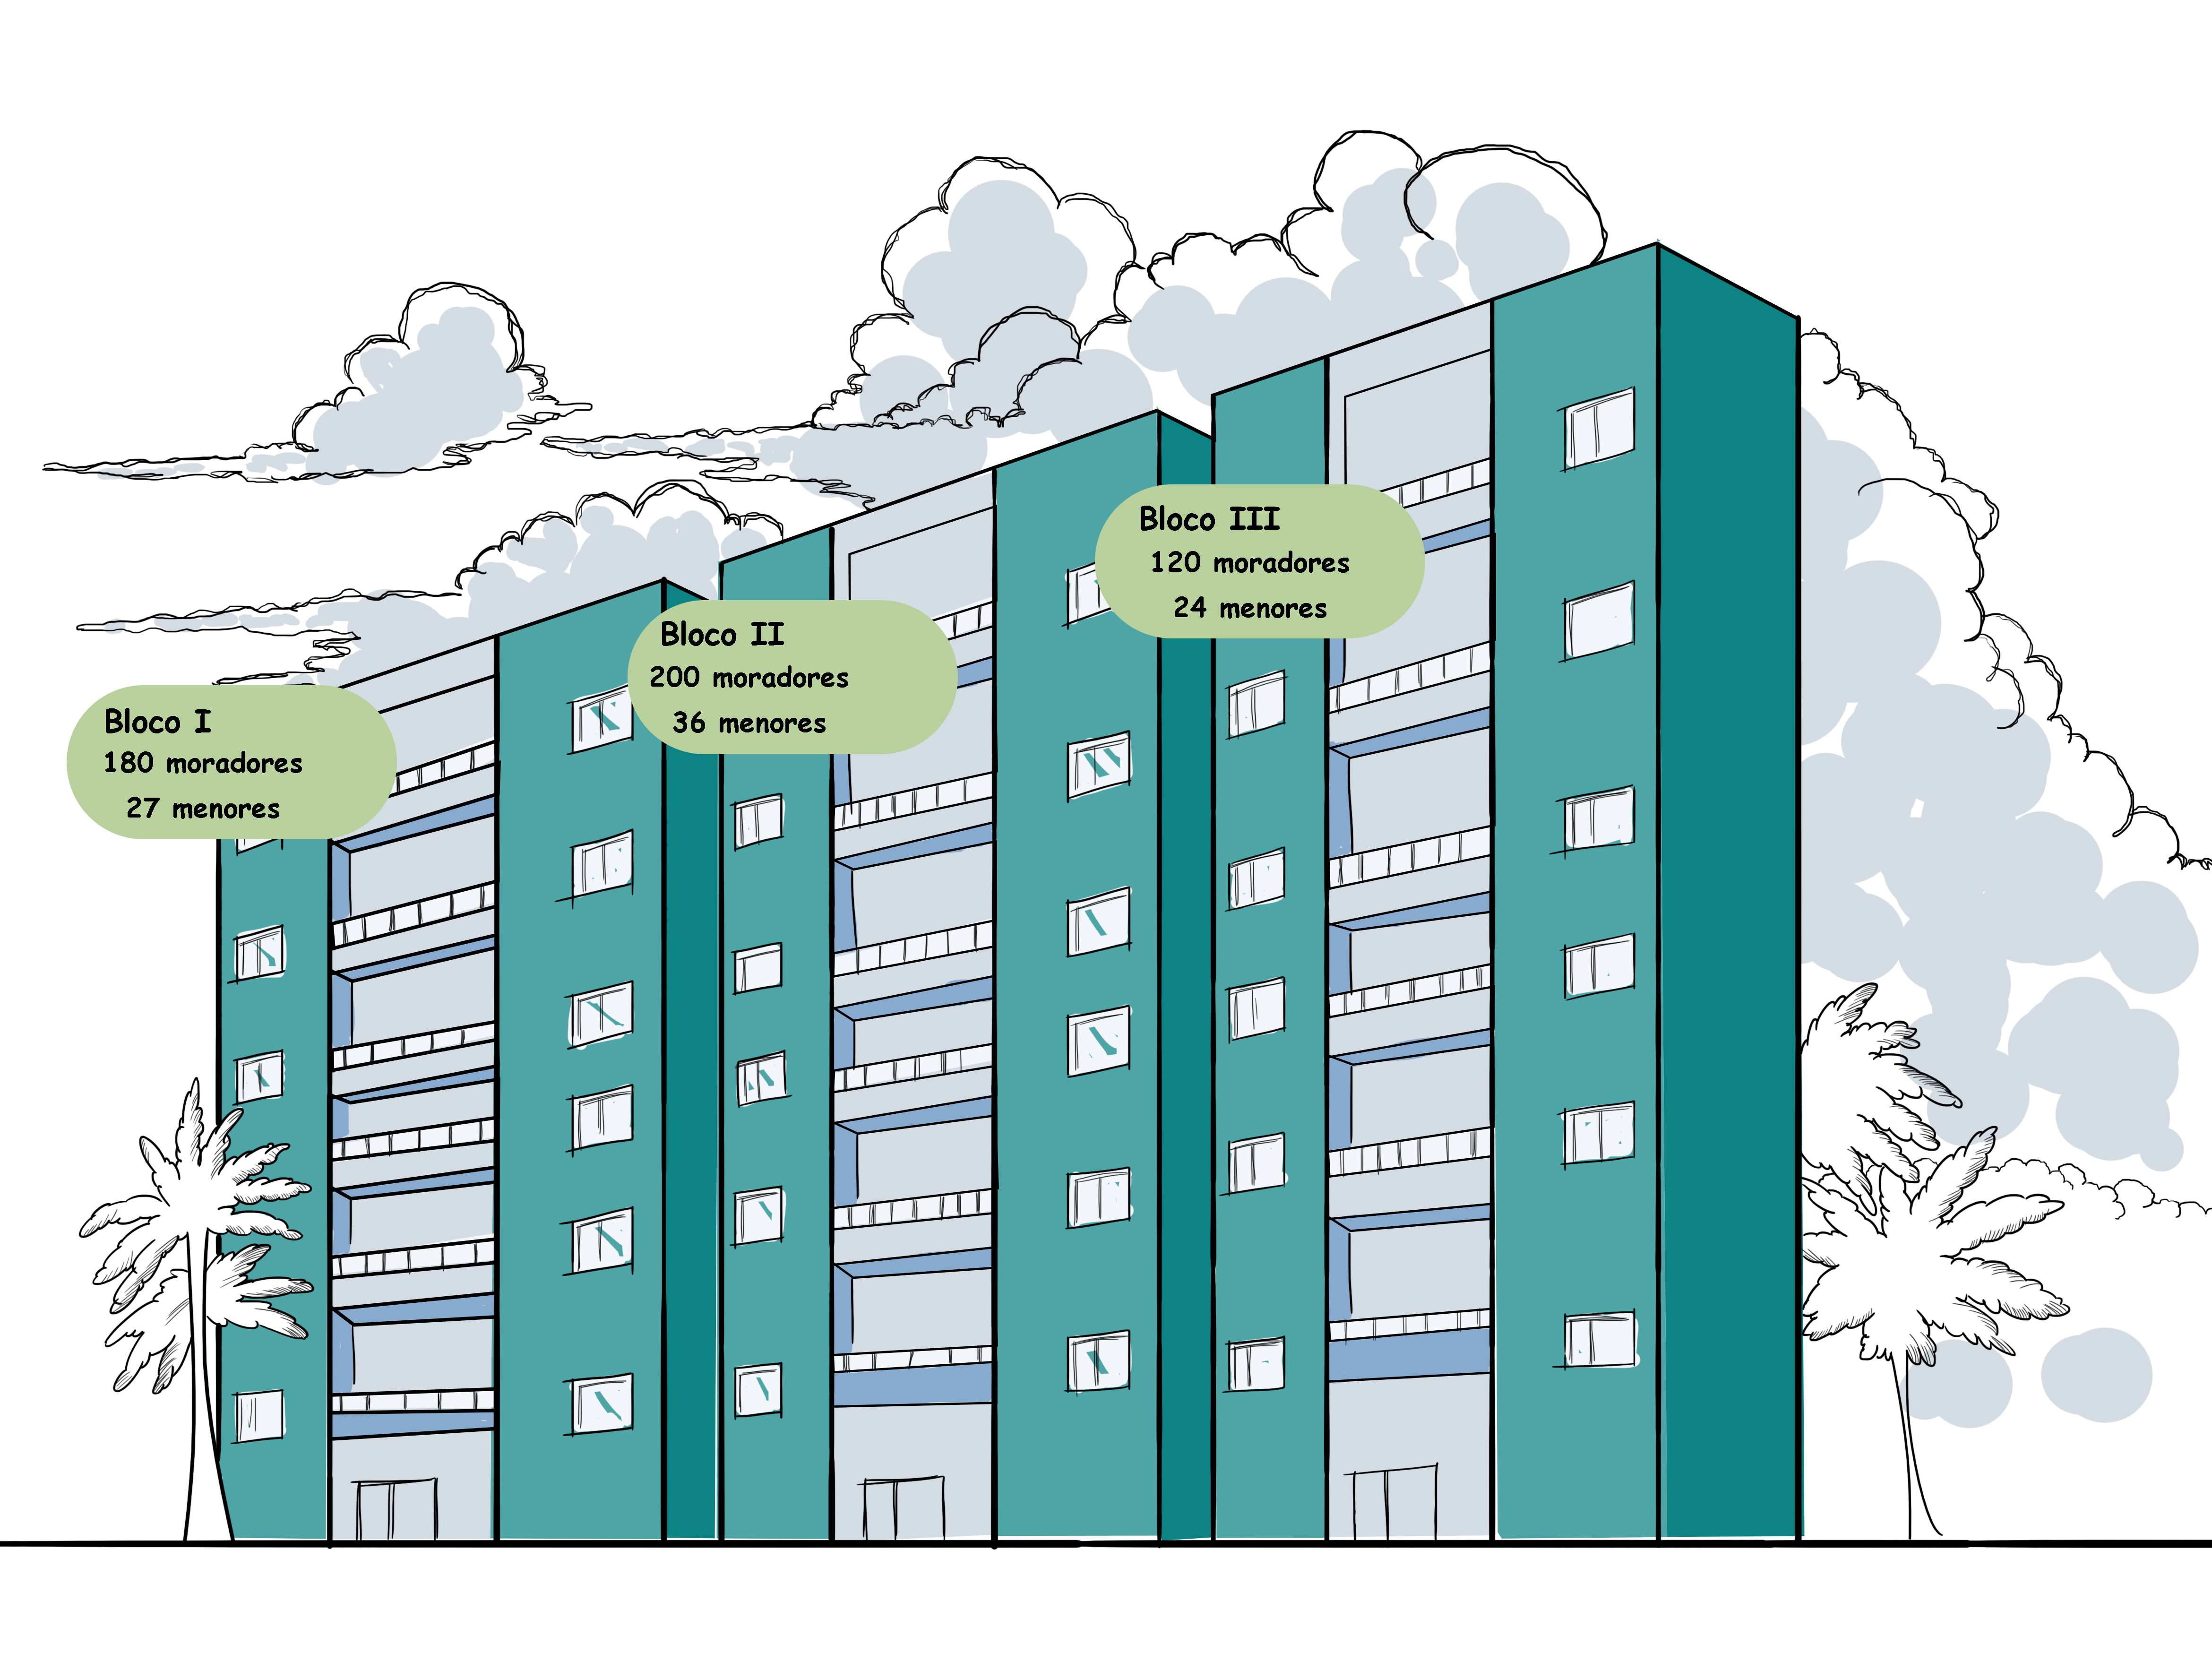
\includegraphics[width=.8\linewidth]{5.jpg}

\caption{Condomínio com três blocos}
\end{figure}

\ifdefined\prof
\begin{solucao}

\begin{enumerate}
\item Defina os seguintes eventos:
\begin{itemize}
\item $A_1$: "bloco I é sorteaco",
\item $A_2$: "bloco II é sorteado" e
\item $A_3$: "bloco III é sorteado".
\end{itemize}
Defina també o evento 
\begin{itemize}
\item B: "um menor de até 12 anos é sorteado". Observe que os eventos $A_1,A_2$ e $A_3$ são disjuntos e que um menor sorteado pode ser de um, e somente um, dos três blocos. Logo, podemos escrever
\begin{equation*}
B=(A_1\cap B)\cup(A_2\cap B)\cup(A_3\cap B).
\end{equation*}
Como os eventos do lado direito da equação acima são disjuntos, tem-se\begin{equation*}
P(B)=(A_1\cap B)+P(A_2\cap B)+P(A_3\cap B)
\end{equation*}
Usando-se a regra da multiplicação, tem-se
\begin{align*}
P(B)&=P(A_1)\cdot P(B|A_1)+P(A_2)\cdot P(B|A_2)+P(A_3)\cdot P(B|A_3)\\
&=\frac{1}{3}+\frac{27}{180}+\frac{1}{3}\cdot\frac{36}{200}+\frac{1}{3}\cdot\frac{24}{100}\\
&=\frac{1}{20}+\frac{3}{50}+\frac{1}{15}\\
&=\frac{15+18+20}{300}\\
&=\frac{53}{300}\approx0{,}177.
\end{align*}

Nesse item, deseja-se calcular a probabilidade condicional de ter ocorrido o evento $A_2$, dado que ocorreu o evento $B$, ou seja, $P(A_2|B)$. Usando a definição de probabilidade condicional tem-se
\begin{align*}
P(A_2|B)&=\frac{P(A_2\cap B)}{P(B)}\\
&=\frac{P(A_2)\cdot P(B|A_2)}{53/300}\\
&=\frac{3}{50}\cdot\frac{300}{53}\\
&=\frac{18}{53}\approx0{,}34.
\end{align*}
\end{itemize}
\end{enumerate}

\end{solucao}
\fi

\end{document}